\documentclass{article}
\usepackage[a4paper, total={6.5in, 9in}]{geometry}
\renewcommand{\contentsname}{Contents}
\usepackage{amssymb}
\usepackage{hyperref}
\usepackage{fancyhdr}
\usepackage{graphicx}
\graphicspath{{./images/}}
\pagestyle{fancy}
\fancyhead{}
\fancyfoot{}
\fancyhead[L]{\slshape\MakeUppercase{Door Alarm System on bare metal Raspberry Pi 4}}
\fancyhead[R]{\slshape Angelo Barbera}
\fancyfoot[C]{\thepage}
\title{\huge Door Alarm System on bare metal Raspberry Pi 4}
\author{Angelo Barbera}
\date{2023}
\begin{document}
\begin{titlepage}
	\centering
	{\scshape\LARGE Unveristà degli studi di Palermo \par}
	\vspace{0.6cm}
	{\scshape\Large Embedded Systems \par}
	\vspace{1.8cm}
	{\huge\bfseries Door Alarm System on bare metal Raspberry Pi 4 \par}
	\vspace{2cm}
	\vfill
	{\large Angelo Barbera 2023 \par}
\end{titlepage}
\newpage
\pagenumbering{roman}
\tableofcontents
\newpage
\clearpage\pagenumbering{arabic}


\section{Introduction}

\section{Hardware}

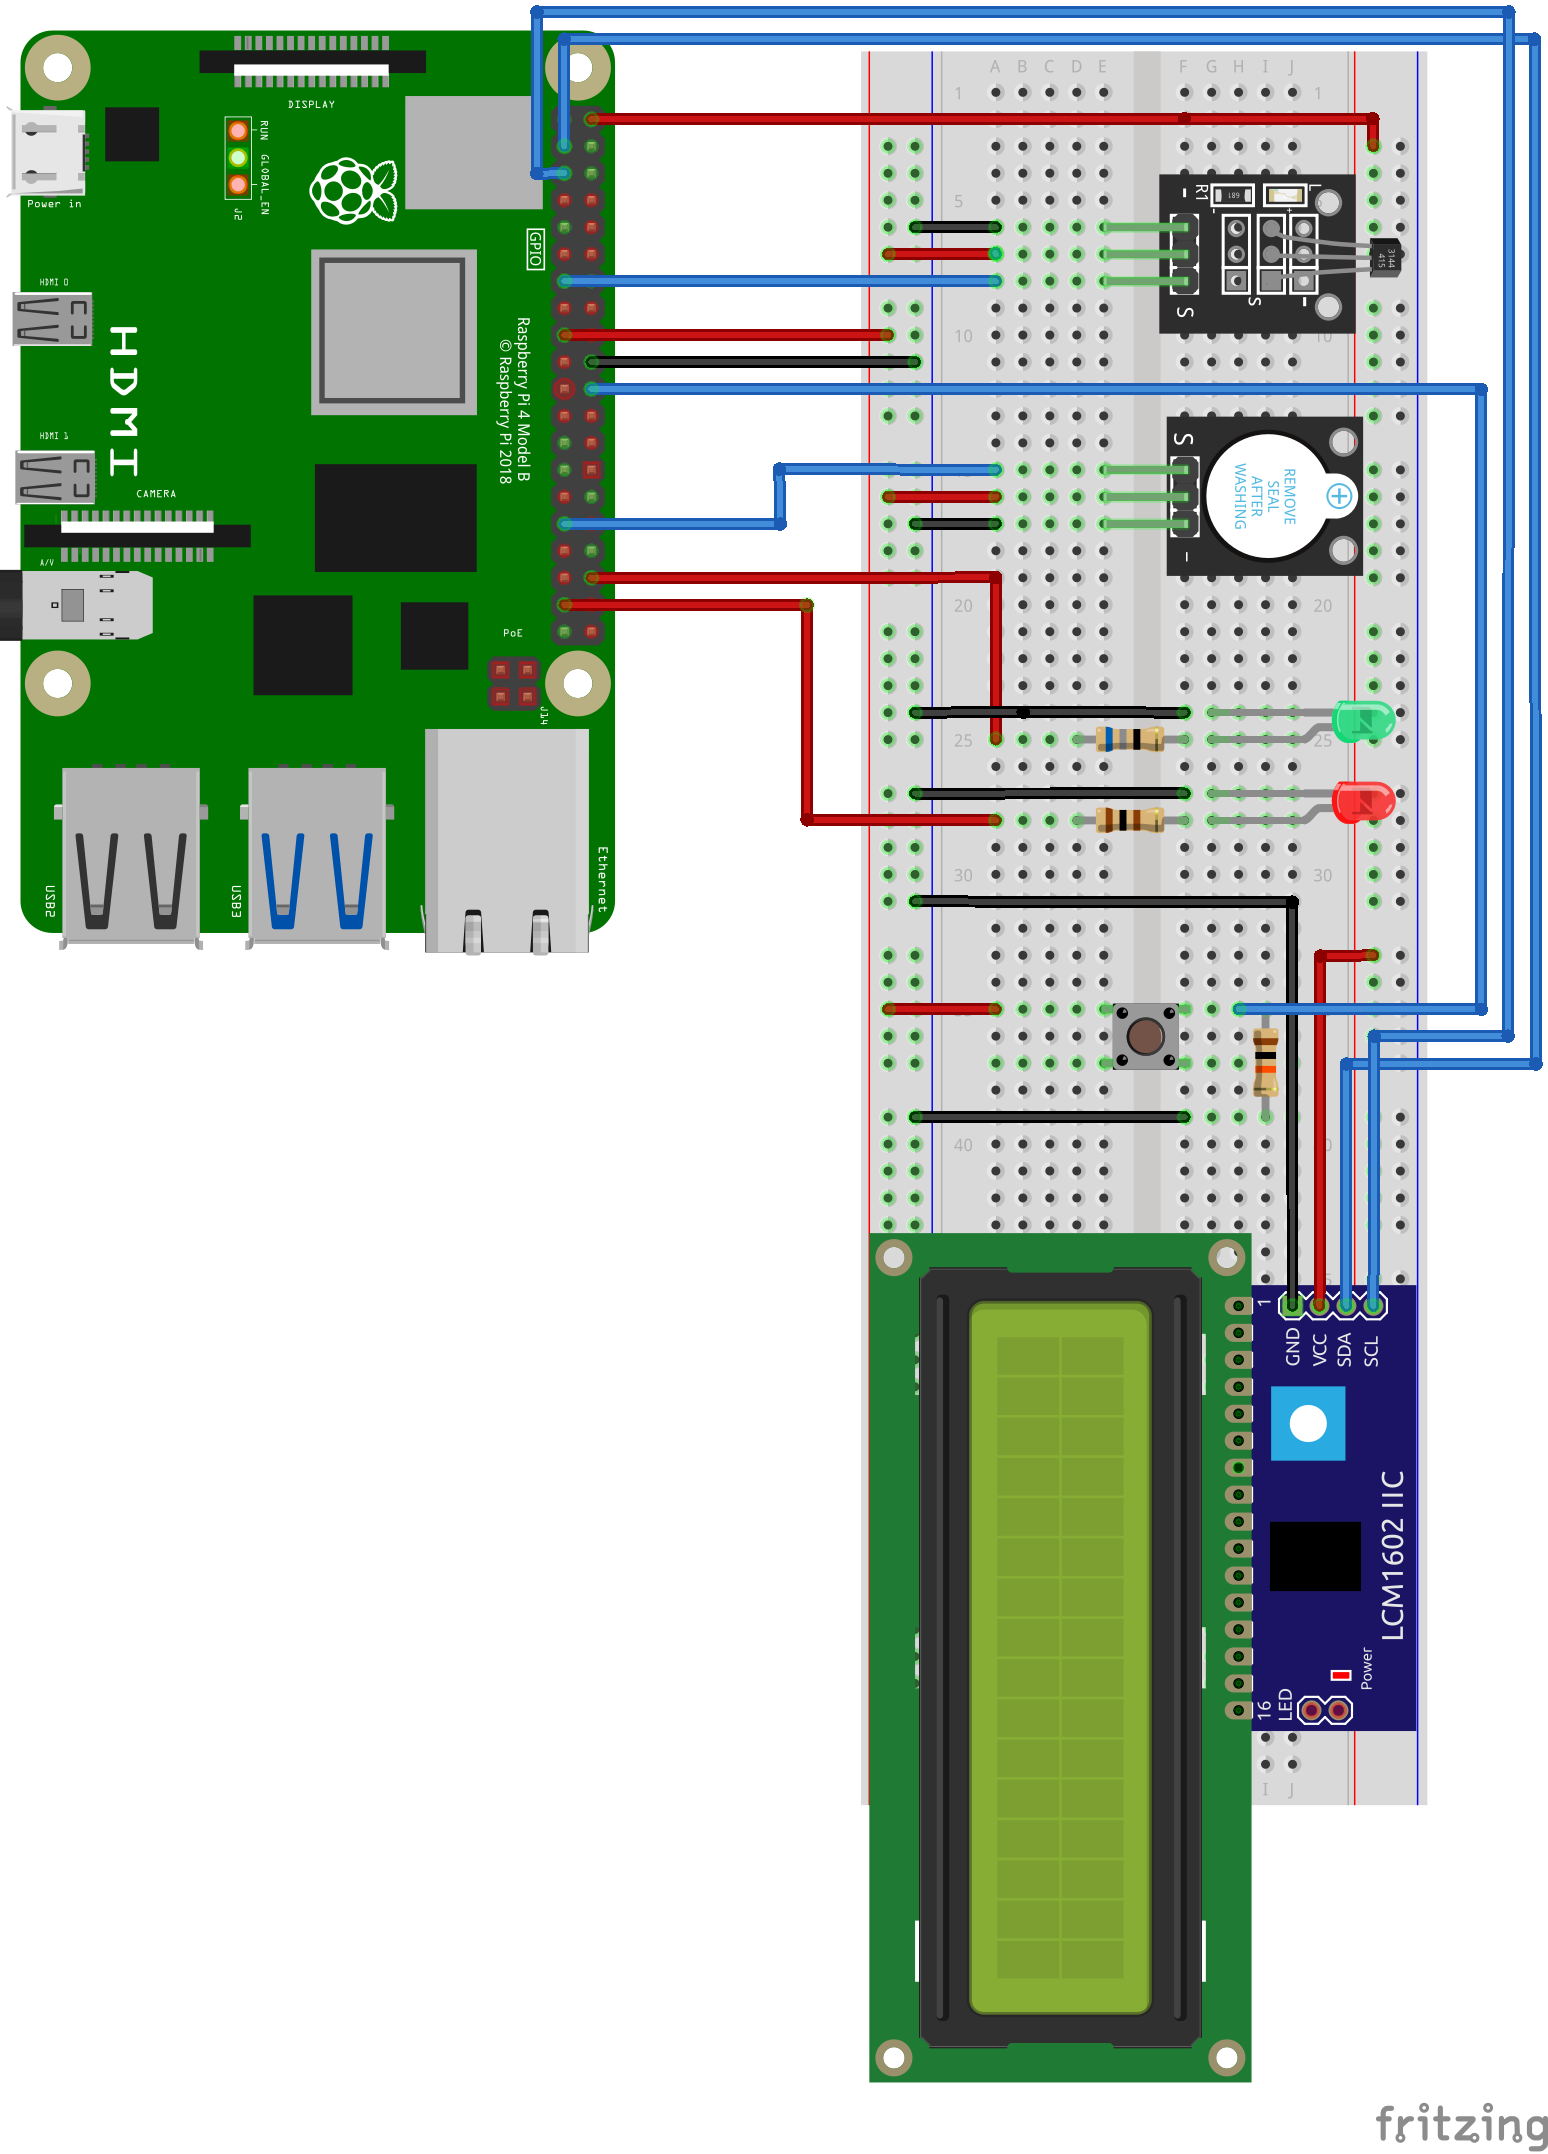
\includegraphics{breadboard.png}

\subsection{Target}
The chosen target for this project is the Raspberry Pi 4 Model B, a single board computer developed by 
the Raspberry Pi Foundation and realeased in 2019.
\\
The tech specs include:
\begin{itemize} 
    \item Broadcom BCM2711, Quad core Cortex-A72 (ARM v8) 64-bit SoC @ 1.5Ghz
    \item 1GB, 2GB, 4GB, or 8GB LPDDR4 SDRAM
    \item 2.4 GHz and 5.0 Ghz 802.11ac wireless
    \item Gigabit Ethernet
    \item Bluetooth 5.0
    \item Two USB 3.0 and two USB 2.0 ports
    \item 40 pin GPIO header
    \item Two micro-HDMI ports up to 4kp60
    \item Micro-SD card slot for loading operating system and data storage
\end{itemize}

\subsection{KY-003 Hall sensor}
The KY-003 hall sensor allow to detect a magnetic field. When the magnetic field at the Hall sensor exceeds
the operate point threshold (BOP) the output of the device switches low. When the magnetic field is reduced
to below the realease point threshold (BRP) the device output switches high.
BOP and BRP may vary respectively from 1 mT to 33 mT and from 5 mT to 35 mT at operating 
temperature T = 25° C depending on the sensor model.
This sensor is used to trigger
the alarm when the  magnetic field detected by the sensor is below the realease point threshold. 

\subsection{LCD 1602}
The LCD 1602 is a liquid crystal display that can display 16x02 characters at the same time. 
This module provides a 16 pin interface and a I2C interface. 
It is used to show the door status (open or closed).

\subsection{KY-012 Buzzer}
The KY-012 Buzzer is an active piezoelectric buzzer, it generates a sound of approximately 2.5kHz when 
input signal (S) is high. The Buzzer is activated when the Hall sensor detect a magnetic field below the BOP

\subsection{LEDs}
When the Hall sensor detects a megnetic field that exceeds the BOP the green LED is on and the red LED is off.
When the Hall sensor detects a megnetic field below the BOP the green LED is off and the red LED is on.

\subsection{Button}
The button is used to turn off the buzzer.

\subsection{Resistors}

\subsection{FT232-AZ USB to TTL serial UART adapter}
The FT232-AZ USB to TTL serial UART adapter is used to connect the PC used during the development of the project
to the target in order to send and receive data between the PC and the Raspberry Pi 4. 
The PC is connected through a USB port, the target is connected through GPIO pins according to the 
following table.

\begin{center}
    \begin{tabular}{ |c|c|c| } 
        \hline
        GPIO \# & Function & UART adapter  \\
        \hline
        14 (Tx) & Output & Rx \\ 
        15 (Rx) & Input & Tx \\ 
        Ground & Ground & Ground \\ 
        \hline
    \end{tabular}
\end{center}

\subsection{GPIO wiring diagram}
The following table is the GPIO wiring diagram.

\begin{center}
    \begin{tabular}{ |c|c|c| } 
        \hline
        GPIO \# & Function & Connection \\
        \hline
        2 & SDA & LCD \\
        3 & SCL & LCD \\
        6 & Output & Buzzer \\
        16 & Output & Green LED \\
        25 & Input & Button \\
        26 & Output & Red LED \\
        27 & Input & Hall sensor \\
        5V & Power & Breadboard \\
        3V3 & Power & Breadboard \\
        Ground & Ground & Breadboard \\
        \hline
    \end{tabular}
\end{center}

\section{Software}


\end{document}